\section{Gravitational Waves}\label{sec:gw_main}
Gravitational waves (\acrshort{gw}s) are a form of radiation, which use spacetime itself as a propagation medium. They are a direct consequence of Albert Einstein's general theory of relativity (\acrshort{gr})~\cite{Einstein:1916aab}, as he found in 1916~\cite{Einstein:1916aaa}. Their effect can be straight forwardly derived assuming only a small deviation from the flat spacetime metric, as will be done in \autoref{sec:linear_gravity}. Sources of \acrshort{gw}s are accelerated masses, or more accurately masses with a non-vanishing second time derivative of their mass-quadrupole moment.

The strength of \acrshort{gw}s depend on the acceleration within the source and the involved masses. The larger the mass and the higher the acceleration, the bigger the amplitude of the resulting wave. For this reason, the sources that can be most easily detected are very heavy objects that experience extreme acceleration. These conditions are fulfilled, for instance, by two very compact astronomical objects, like black holes (\acrshort{bh}s) or neutron stars (\acrshort{ns}), that rapidly orbit each other.

Over time, a binary system of compact objects loses energy, due to the emission of gravitational radiation. This causes the two bodies to slowly come closer together until they merge. \acrshort{gw} signals emitted by systems of this kind are known as \emph{compact binary coalescence} (\acrshort{cbc}) signals and they are usually classified into three categories; binary neutron stars (\acrshort{bns}), binary black holes (\acrshort{bbh}s), and \acrshort{ns}-\acrshort{bh}-systems (\acrshort{nsbh}). At the time of writing this thesis, all $\mathcal{O}\lr{100}$ detected \acrshort{gw}s are believed to belong to one of these classes~\cite{LIGOScientific:2021djp, Nitz:2021zwj}. 

\acrshort{cbc}-signals are commonly described to be composed of three stages; the \emph{inspiral}, the \emph{merger}, and the \emph{ringdown}. During the initial phase, the two bodies have a large separation and relativistic effects are small. The resulting \acrshort{gw}s can be well described by analytic approximations, an overview of which is given in \autoref{sec:linear_gravity} and \autoref{sec:pn}. This phase is known as the inspiral, as the two objects are slowly spiraling towards each other, due to the orbital energy carried away by the emitted \acrshort{gw}s. During the final few orbits relativistic effects have a non-negligible effect on the orbital dynamics and the approximations made during the inspiral phase are not valid anymore. Because the two bodies merge in this phase, it is called the merger. For accurate descriptions of the \acrshort{gw} during this phase one has to resort to numerical relativity~\cite{Maggiore:2008aaa}. %page 237
Their discussion goes beyond the scope of a brief introduction and I refer the interested reader to section 14.3 of \cite{Maggiore:2018aaa} for an introduction to the topic and to \cite{Pretorius:2007nq, Hannam:2009rd, Hinder:2010vn, Centrella:2010zf} for deeper reviews. Once the binary has merged, the resulting body is a perturbed compact object. This perturbation will then be radiated off during the ringdown phase~\cite{Nollert:1999ji} which for \acrshort{bh}s can be described analytically and yields exponentially damped sinusoids~\cite{Nollert:1999ji}. When the remnant is some kind of \acrshort{ns} the ringdown is affected by the mass distribution and can be a lot more complicated~\cite{Bauswein:2012ya}. I will not discuss the ringdown in this work, but will point the interested reader to \cite{Kokkotas:1999bd}.

Other kinds of \acrshort{gw} sources are expected to exist but have not yet been directly detected. The most promising candidates for future detection include continuous gravitational waves (\acrshort{cw})~\cite{Dergachev:2020fli, Steltner:2020hfd, LIGOScientific:2022pjk}, supernovae (\acrshort{sn})~\cite{LIGOScientific:2016jvu}, and extreme mass ratio inspirals (\acrshort{emri})\cite{Maggiore:2018aaa, LISA:2017pwj}. %page 339
 \acrshort{cw}s are emitted by a rapidly spinning \acrshort{ns} whose shape slightly deviates from that of a perfect sphere. If the deformation is not rotationally symmetric around the rotation axis of the star, it causes the second time derivative of the quadrupole moment to be non-zero. Due to the extreme stability of the rotational frequency of observed \acrshort{ns}~\cite{Matsakis:1997aaa, Verbiest:2009aaa} and the low amount of energy lost due to emitted \acrshort{gw}s, the signal is expected to have a very small amplitude, but be extremely long lasting and almost monochromatic~\cite{Lasky:2015uia}. \acrshort{sn} can emit \acrshort{gw}s due to the rapid evolution of their mass distribution and the scales of energy which are released during their explosion. The exact mechanisms that lead to the emission of gravitational radiation are manifold and can only be modeled numerically~\cite{Maggiore:2018aaa}. %Chapter 10
\acrshort{emri}s are binary systems, where one object is of stellar mass, such as a \acrshort{ns}, stellar mass \acrshort{bh}, or white dwarf (\acrshort{wd}), while the other body is a supermassive black hole (\acrshort{smbh}). In this setup, the mass ratio between the two bodies is on the order $\geq 10^5$ and most established methods to calculate the emitted \acrshort{gw}s break down~\cite{Maggiore:2018aaa}. %page 343
However, we do expect to be able to detect \acrshort{emri}s with future, space-born detectors~\cite{LISA:2017pwj}. While these signals are expected to exist, this thesis will exclusively treat \acrshort{cbc} signals.

Even the strongest \acrshort{gw}s interact only very weakly with matter and other forms of energy~\cite{Maggiore:2008aaa}. %page 23, eq (1.96): forces are small -> energy transfer small (work)
For this reason they travel almost unaffected through the Universe. This is a major advantage over electromagnetic (\acrshort{em}) radiation, which is shielded by matter, and is especially important when studying the very early stages of the Universe, where it was opaque to \acrshort{em} radiation~\cite{Ratra:2007sa}. Additionally, the most common sources observed today are very compact objects which usually do not emit a lot of \acrshort{em} radiation. Studying them through \acrshort{gw}s allows us to detect them nonetheless and make statements about their population~\cite{LIGOScientific:2021psn}, constrain the percentage of dark matter that can be explained by \acrshort{bh}s~\cite{LIGOScientific:2021job}, and test \acrshort{gr}~\cite{LIGOScientific:2016lio, LIGOScientific:2021sio}.

Subsection \ref{sec:linear_gravity} closely follows sections 2.1.1 of \cite{Schaefer:2019:MSC}. Subsection \ref{sec:pn} is oriented along chapter 5 of \cite{Maggiore:2008aaa} and \cite{Blanchet:2006aaa}. Throughout this section I will use the Einstein summation convention, denote 4-dimensional spacetime indices by Greek letters, and purely spatial indices by Latin letters. The convention $\eta^\mn=\text{diag}\lr{-, +, +, +}$ is used for the flat special relativistic Minkowski-metric.

\subsection{Linearized Gravity}\label{sec:linear_gravity}
In \acrshort{gr} gravity is described as a property of spacetime. Instead of being a force, gravity is the effect of following shortest paths in a curved spacetime. The curvature is governed by the Einstein equation
\begin{equation}\label{eq:einstein}
\mathcal{G}_\mn = \frac{8\pi G}{c^4}T_\mn,
\end{equation}
where $\mathcal{G}_\mn$ is the Einstein tensor, $G$ is the gravitational constant, $c$ is the speed of light in vacuum, and $T_\mn$ is the energy-momentum tensor. $\mathcal{G}_\mn$ is constructed entirely from constants and a combination of the spacetime metric $g_\mn$ and its first and second derivatives. Overall, \eqref{eq:einstein} specifies a set of coupled, non-linear, second order, partial differential equations, where $T_\mn$ acts as the source of the curvature. To find trajectories of test-particles in this theory, one needs to specify the matter-, energy-, and stress-contents of the universe in the energy-momentum tensor $T_\mn$. Afterward, the set of differential equations have to be solved to find the metric $g_\mn$. From the metric one can then find (local) trajectories by solving the geodesic equation
\begin{equation}\label{eq:geodesic_equation}
\ddot{x}^\rho + \Gamma^\rho_\mn\dot{x}^\mu\dot{x}^\nu = 0,
\end{equation}
where $\Gamma^\rho_\mn$ are Christoffel-symbols and $\dot{x}^\mu$ is the derivative of $x^\mu$ by the proper time.

As stated earlier, \acrshort{gw}s are waves that use spacetime as their medium. In mathematical terms, we are looking for a wave-like solution $g_\mn$ to the Einstein equation \eqref{eq:einstein}. Their existence in \acrshort{gr} should not be surprising, as one of the core concepts of the theory is that nothing travels faster than light in vacuum. As a result the curvature changes induced by moving masses will also have to obey this speed limit. Analogously, in electrodynamics electric charges act as a source of the electric field, which travels at the speed of light. When they are accelerated, one finds wave-like solutions to the field equations. Therefore, a waveform solution to the Einstein equation seems plausible from a physical standpoint.

To find these solutions we assume small and slowly varying deviations from a flat spacetime. In mathematical terms we are only considering metrics
\begin{equation}\label{eq:linear_metric}
g_\mn = \eta_\mn + h_\mn,
\end{equation}
with $\left|\left|h_\mn\right|\right|\ll 1$ and $\left|\left|\partial_{\sigma_1}\dots\partial_{\sigma_n}h_\mn\right|\right|\in\mathcal{O}\lr{h_\mn}\eqqcolon\mathcal{O}\lr{h}$. Inserting \eqref{eq:linear_metric} into \eqref{eq:einstein} and keeping only terms linear in $h_\mn$ and its derivatives, i.e. discarding any terms of order $\mathcal{O}\lr{h^2}$ and above, yields the linearized Einstein equation
\begin{equation}\label{eq:einstein_linear}
\mathcal{G}_\mn = \frac{1}{2} \lr{\partial_{\alpha\mu}h^\alpha_\nu + \partial^\alpha_\nu h_{\mu\alpha} - \partial_\mn h - \Box h_\mn - \eta_\mn \partial^{\sigma\alpha}h_{\sigma\alpha} + \eta_\mn\Box h} = \frac{8\pi G}{c^4}T_\mn,
\end{equation}
where $h\coloneqq \eta^\mn h_\mn$ and $\Box\coloneqq \eta^\mn\partial_\mn$.

The linearized Einstein equation is invariant under coordinate transformations $x_\mu'=x_\mu + \xi_\mu\lr{x}$, when $\left|\left|\partial_\mu\xi_\nu\right|\right|\in\mathcal{O}\lr{h}$~\cite{Maggiore:2008aaa}. We can use this property\footnote{See \cite{Wald:1984aaa} for a more mathematical justification of this gauge freedom.%page 75
} to choose a gauge condition that simplifies the equation. To simplify notation we can define $\bar{h}_\mn\coloneqq h_\mn-\frac{1}{2} \eta_\mn h$. We can then use the DeDonder gauge~\cite{Maggiore:2008aaa}
\begin{equation}
\partial^\alpha\bar{h}_{\alpha\mu} = 0,
\end{equation}
by choosing $\Box\xi_\mu = \partial^\alpha\bar{h}_{\alpha\mu}$, which is known to always have a solution~\cite{Maggiore:2008aaa}. %page 7
In this gauge equation \eqref{eq:einstein_linear} reduces to
\begin{equation}\label{eq:wave_eq_hbar}
\Box\bar{h}_\mn = -\frac{16\pi G}{c^4}T_\mn.
\end{equation}
This equation is a well known wave equation~\cite{Dragon:2016aaa}, which, again, is known to always have a solution. However, the DeDonder gauge doesn't fix the coordinate system completely. It only used $\Box\xi_\mu = \partial^\alpha\bar{h}_{\alpha\mu}$, which was set to zero. Other transformations with $\Box\xi_\mu=0$ are still allowed. This freedom can be used to further constrain the degrees of freedom of \eqref{eq:wave_eq_hbar}. It allows us to set the trace of the metric perturbation $h=0$. As a consequence $\bar{h}_\mn = h_\mn$. It also allows us to set the components $h_{0\mu} = 0 = h_{3\mu}$, by choosing the coordinate system such that the wave-vector of the solution points in the $x_3$-direction~\cite{Misner:1973aaa}. %page 947
In this gauge, solutions must be of the form
\begin{equation}
h^{\text{\acrshort{tt}}}_\mn=
\begin{pmatrix}
	0 & 0         & 0        & 0\\
	0 & h_+       & h_\times & 0\\
	0 & h_\times & -h_+      & 0\\
	0 & 0         & 0        & 0\\
\end{pmatrix}.
\end{equation}
By construction in this gauge the metric is traceless and transverse in nature, i.e. $k^\mu h_\mn=0$ where $\vec{k}$ is the wave-vector \cite{Misner:1973aaa}. %page 947
For this reason it is known as the \emph{transverse-traceless gauge} (\acrshort{tt}). The superscript \acrshort{tt} specifies that the metric is evaluated in the \acrshort{tt} gauge.

A complete gauge, such as the \acrshort{tt} gauge, selects one specific coordinate system. It is usually chosen to simplify calculations, but may not be observable. To understand the coordinate system chosen by the gauge conditions underlying the \acrshort{tt} gauge, we can check the trajectories of test particles which are initially at rest ($\dot{x}^i=0$) in this frame. In this case, the geodesic equation \eqref{eq:geodesic_equation} simplifies to~\cite{Maggiore:2008aaa}%page 17
\begin{equation}
\ddot{x}^i = -\Gamma^i_{00}\lr{\dot{x}^i}^2=-\frac{1}{2}\lr{2\partial_0 h_{0i}-\partial_i h_{00}}\lr{\dot{x}^i}^2 \overset{\text{\acrshort{tt}}}{=} 0.
\end{equation}
Therefore, particles at rest remain at rest and are not accelerated by the passing of a \acrshort{gw}. This means that the reference frame selected by the \acrshort{tt} gauge changes with the \acrshort{gw}.

However, the coordinate system of the \acrshort{tt} gauge is not the frame we observe. Instead, we observe from a central point and live in a locally flat spacetime. Mathematically this can be expressed by constructing a local inertial frame at a point chosen as the origin and describing everything in terms of that frame~\cite{Maggiore:2008aaa}. %page 15
To calculate the change in the distance of any point from the origin, we can use the equation for the geodesic deviation, which reduces to
\begin{equation}\label{eq:geodesic_deviation_simple}
\ddot{x}^i = -R_{i 0 j 0} x^j
\end{equation}
in linearized gravity and this frame of reference~\cite{Misner:1973aaa}. %page 950/951
$R_{\mu\nu\sigma\rho}$ is the Riemann tensor, which is invariant under coordinate transformations in linearized gravity~\cite{Maggiore:2008aaa}. %page 6 and 18
We can, therefore, choose any gauge we like to calculate it. In the \acrshort{tt} gauge the required components are given by $R_{i0j0} = -\frac{1}{2c^2}\ddot{h}^{\text{\acrshort{tt}}}_{ij}$. Inserting this expression into \eqref{eq:geodesic_deviation_simple} one can directly integrate the equation to get~\cite{Misner:1973aaa}% page 951
\begin{equation}\label{eq:geodesic_deviation_gw}
x^i\lr{\tau} = x^j\lr{0}\lr{\delta_{ij} + \frac{1}{2}h^{\text{\acrshort{tt}}}_{ij}\lr{\tau}}.
\end{equation}

In this frame we can then observe the effect of a passing \acrshort{gw} on a ring of freely falling test-masses in the $x$-$y$-plane. To obtain a solution to \eqref{eq:wave_eq_hbar} we assume to be in vacuum, i.e. $T_\mn=0$. One special solution to this equation is the plane wave $h^{\text{\acrshort{tt}}}_{ij} = A_{ij}\sin\lr{\omega\tau}$. The effect of such a solution on the ring of test-masses for the two individual polarizations as obtained from \eqref{eq:geodesic_deviation_gw} is depicted in \autoref{fig:effect_gw}. The figure justifies the names ``plus'' and ``cross'' given to the two polarizations $h_+$ and $h_\times$, respectively.

\begin{figure}
	\centering
	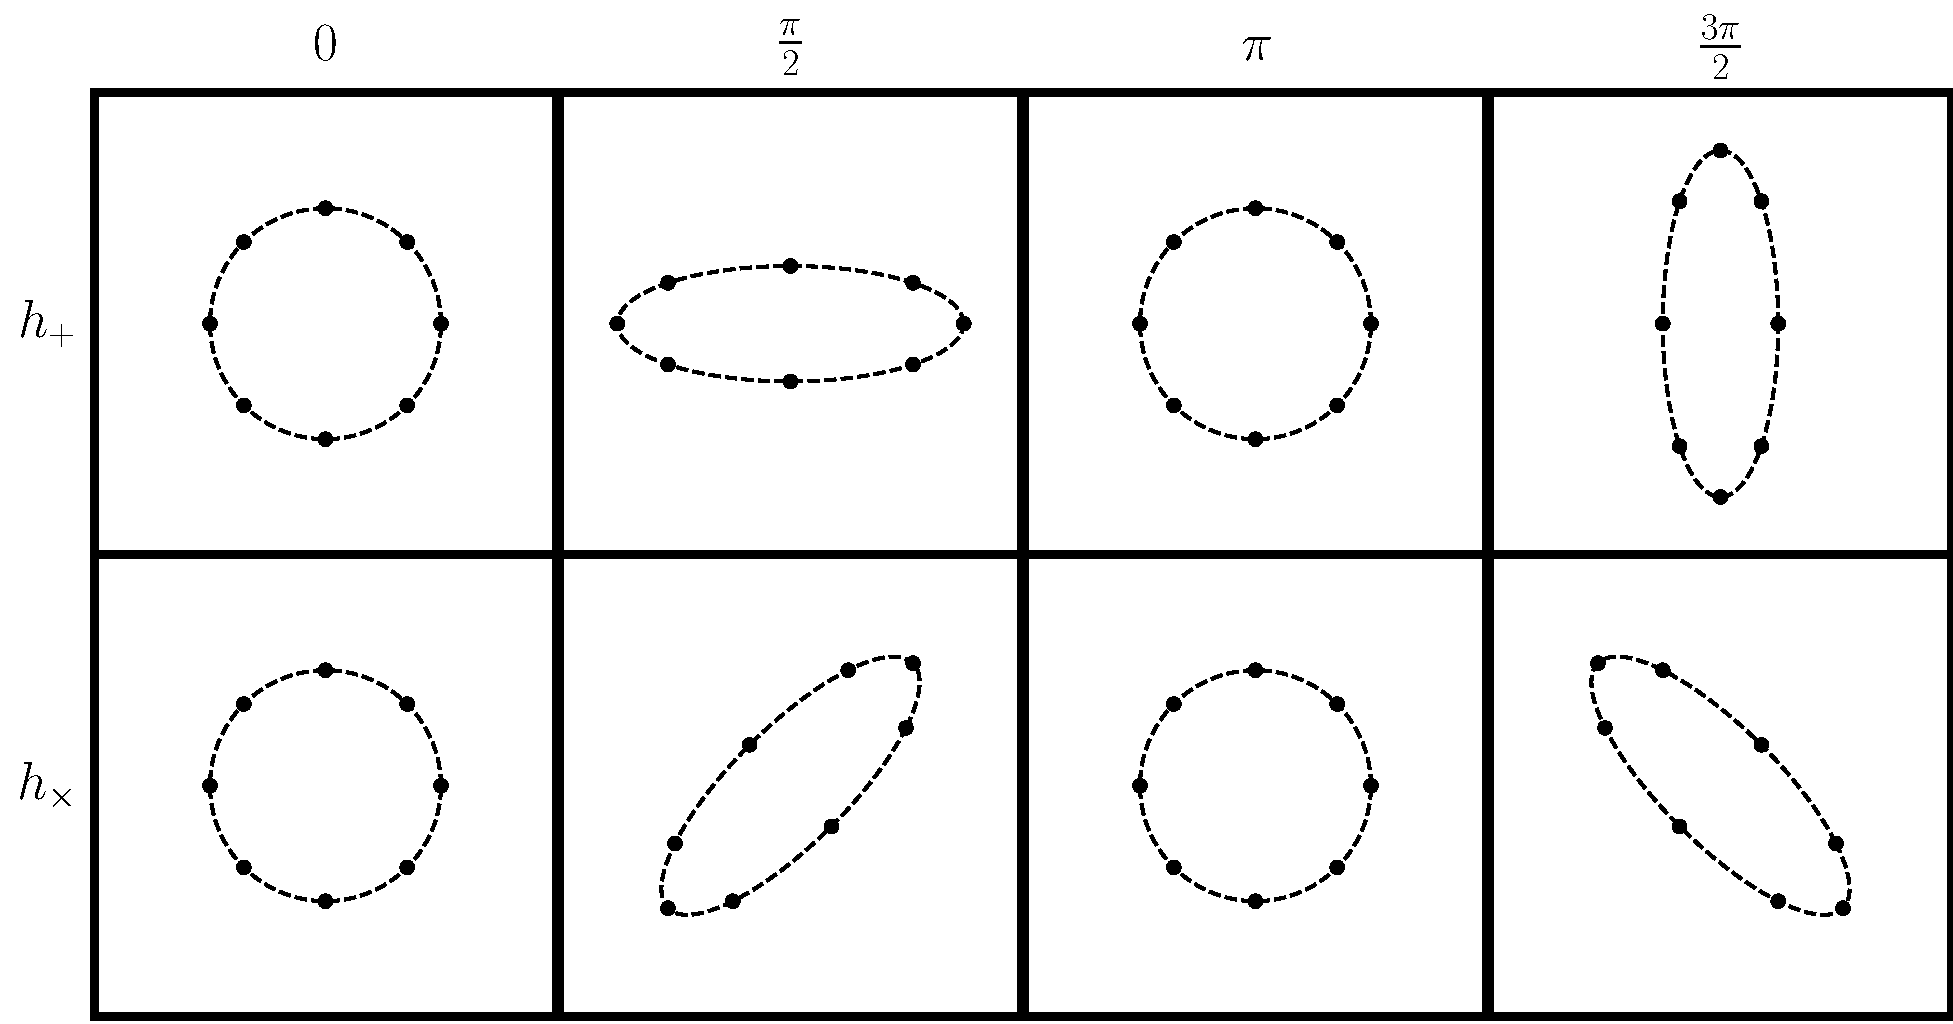
\includegraphics[width=\textwidth]{chapters/foundations/sections/gw/images/effect_gw.pdf}
	\caption[Effect of a gravitational wave on a ring of test-masses]{The effect of a \acrshort{gw} on a ring of freely falling test masses in the plane perpendicular to the propagation direction of the \acrshort{gw}. The two rows show the effect of the ``plus'' and ``cross'' polarization, respectively. The columns show different phases of the wave. The labels give the value of $\omega\tau$.}\label{fig:effect_gw}
\end{figure}

While the observable effects of a \acrshort{gw} can be studied by assuming vacuum solutions, their production cannot. To do so, the general solution of equation \eqref{eq:wave_eq_hbar} has to be considered, which is given by
\begin{equation}\label{eq:wave_solution_general}
\bar{h}_\mn\lr{t,\vec{x}}=\frac{4G}{c^4}\int \Diff{3}x'\ \frac{T_\mn\lr{t-\left|\left|\vec{x}-\vec{x}'\right|\right| /c,\vec{x}'}}{\left|\left|\vec{x}-\vec{x}'\right|\right|}.
\end{equation}
As the approximations underlying linearized gravity are only valid when there are at most small deviations from flat spacetime, we consider \eqref{eq:wave_solution_general} only far from the source of radiation. At large distances to the source the scale within the source is negligible and as such $\norm{\vec{x}-\vec{x}'}\approx\norm{\vec{x}}\eqqcolon r$. Using this approximation \eqref{eq:wave_solution_general} simplifies to
\begin{equation}
\bar{h}_\mn\lr{t,\vec{x}}=\frac{4G}{c^4}\frac{1}{r}\int \Diff{3}x'\ T_\mn\lr{t-r/c, \vec{x}'}.
\end{equation}
Projecting the equation into the \acrshort{tt} gauge and using that the energy-momentum tensor is divergence free, one finds~\cite{Maggiore:2008aaa}%page 109
\begin{equation}\label{eq:quadrupole-formula}
h^{\text{\acrshort{tt}}}_{ij}\lr{t, \vec{x}} = \frac{2G}{c^4}\frac{1}{r}\ddot{I}^{\text{\acrshort{tt}}}_{ij}\lr{t-r/c},
\end{equation}
where $\ddot{I}^{\text{\acrshort{tt}}}_{ij}$ is the second time derivative of the projection into the \acrshort{tt} gauge of the second mass moment
\begin{equation}
\ddot{I}^{ij} = c^2 \partial^2_0\int\Diff{3}x'\ x'^ix'^j T^{00}.
\end{equation}
The projection of this quantity is given by~\cite{Maggiore:2008aaa}%page 110
\begin{equation}\label{eq:I-tt-projection}
\ddot{I}^{\text{\acrshort{tt}}}=
\begin{pmatrix}
\lr{\ddot{I}_{11}-\ddot{I}_{22}}/2 & \ddot{I}_{12} & 0\\
\ddot{I}_{21} & -\lr{\ddot{I}_{11}-\ddot{I}_{22}}/2 & 0\\
0 & 0 & 0
\end{pmatrix}.
\end{equation}

The above equations can be used to approximate the gravitational radiation emitted by any mass distribution. Because this work considers only \acrshort{cbc} sources, we are interested in the \acrshort{gw}s sent out by two point particles orbiting each other. Due to the initial assumptions of linearized gravity, we are restricted to a separation of the two objects where the curvature of the background spacetime caused by the other object is small. In turn, however, this means that the orbital dynamics are governed by Newtonian dynamics and the problem reduces to the Kepler problem~\cite{Maggiore:2008aaa}. %page 120, 158
One solution to this problem are circular orbits, which can be described using an effective one body formalism with the reduced mass $\mu=\frac{m_1 m_2}{m_1 + m_2}$. From this setup the second time derivative of the second mass moment is calculated to be
\begin{equation}\label{eq:I-binary-point-masses}
\ddot{I}^{ij}=2\mu R^2 {\omega_s}^2
\begin{pmatrix}
\cos\lr{2\omega_s t} & \sin\lr{2\omega_s t} & 0\\
\sin\lr{2\omega_s t} & -\cos\lr{2\omega_s t} & 0\\
0 & 0 & 0
\end{pmatrix},
\end{equation}
where $R$ is the orbital separation of the two bodies and $\omega_s$ is their orbital frequency. In combination with \eqref{eq:quadrupole-formula} and \eqref{eq:I-tt-projection} this can be used to find the expressions for the polarizations of the \acrshort{gw}s. Interestingly, the frequency of \acrshort{gw}s originating from a binary system in circular orbits is exactly twice the orbital frequency. For eccentric orbits this property is lost \cite{Maggiore:2008aaa}.%page 182

The expressions obtained from the system described by \eqref{eq:I-binary-point-masses} are given in the frame of reference used to solve the Kepler problem. This means that we obtained the waves emitted in the $x^3$ direction from the center of mass. However, we are interested in the radiation emitted in all directions, as we cannot a priori know the orientation of a source with respect to our detectors. To resolve this issue, one needs to do one final projection which yields the waveform functions~\cite{Maggiore:2008aaa}%page 111
\begin{align}\label{eq:circular_orbit_waveforms}
h_+ & = \frac{4}{r}\frac{G}{c^4}\mu R^2 {\omega_s}^2\lr{\frac{1+\cos^2\lr{\iota}}{2}}\cos\lr{2\omega_s t + 2 \Phi}\nonumber\\
h_\times & = \frac{4}{r}\frac{G}{c^4}\mu R^2 {\omega_s}^2\cos\lr{\iota}\sin\lr{2\omega_s t + 2 \Phi},
\end{align}
where $\iota$ is the inclination of the system with respect to the line of sight and $\Phi$ is the orbital phase of the two objects at $t=0$.

Equation \eqref{eq:geodesic_deviation_gw} showed that \acrshort{gw}s can change the distance between particles. Therefore, the particles obtain kinetic energy from a passing \acrshort{gw} and stress can be induced in rigid bodies~\cite{Maggiore:2008aaa}. %page 26
As a consequence, \acrshort{gw}s must carry energy in order to pass it on. However, according to \eqref{eq:einstein}, if \acrshort{gw}s carry energy, they must act as a source of curvature themselves and the assumption \eqref{eq:linear_metric} of \acrshort{gw}s being a small perturbation in a flat background is not sufficient anymore. Instead one needs to consider a more general metric $g_\mn=\hat{g}_\mn+h_\mn$.

To obtain the energy carried by a \acrshort{gw} the background $\hat{g}_\mn$ must be separated from the \acrshort{gw} $h_\mn$. To achieve this we impose the condition that the background curvature fluctuates at most slowly compared to the rapidly oscillating $h_\mn$. In a rather lengthy calculation one can expand the Ricci tensor in terms of $h_\mn$ to second order. Taking the time average over multiple cycles of the \acrshort{gw} will then filter out its contribution to the curvature and leaves the background curvature behind. However, since terms quadratic in $h_\mn$ may have low frequency components, when the wave-vectors $\vec{k}_1$ and $\vec{k}_2$ are of similar magnitude but opposite sign, one can find that the \acrshort{gw} does have an influence on the background curvature. Since the background changes very slowly compared to the \acrshort{gw}, we can again view it as locally flat. Under these assumptions one can then write down an expression for the effective energy-momentum tensor of a \acrshort{gw}
\begin{equation}
t_\mn=\frac{c^4}{32\pi G}\langle\partial_\mu \lr{h^{\text{\acrshort{tt}}}}^{\sigma\alpha}\partial_\nu h^{\text{\acrshort{tt}}}_{\sigma\alpha}\rangle .
\end{equation}
A more thorough discussion of this derivation can be found in 1.4.2 of \cite{Maggiore:2008aaa}, where most of the above was paraphrased from, and 35.13 and 35.15 of \cite{Misner:1973aaa}.

Due to conservation of energy, the energy carried by the \acrshort{gw} must be taken away from the source. The main form of energy stored in the binary system studied above is the orbital energy. In turn, this means that the assumption of a constant circular orbit that led to the equations \eqref{eq:circular_orbit_waveforms} cannot hold. Instead one needs to consider the energy lost by gravitational radiation to calculate the phase of the \acrshort{gw}. 

The total energy carried away from the system is known as the luminosity and can be obtained by integrating the outwards pointing energy flux over a sphere with infinite radius. If we consider a binary system with large separation, where the orbital dynamics are well approximated by Newtonian theory, one finds
\begin{equation}\label{eq:luminosity_linear}
L_{\text{\acrshort{gw}}}=\frac{32}{5}\frac{c^5}{G}\lr{\frac{G\omega_s M_c}{c^3}}^{10 / 3}
\end{equation}
for the luminosity $L_{\text{\acrshort{gw}}}$, where
\begin{equation}
M_c\coloneqq \frac{\lr{m_1 m_2}^{3/5}}{\lr{m_1 + m_2}^{1/5}}
\end{equation}
is the chirp mass.

By setting the change in orbital energy equal to the luminosity and using Kepler's third law one can obtain a differential equation of the orbital frequency. This can be solved to get~\cite{Maggiore:2008aaa}%page 170
\begin{equation}
f_{\text{\acrshort{gw}}}\lr{\tau}=\frac{1}{\pi}\lr{\frac{5}{256}\frac{1}{\tau}}^{3/8}\lr{\frac{G M_c}{c^3}}^{-5/8},
\end{equation}
where $\tau$ is the time until the system merges. Integration yields the orbital phase
\begin{equation}
\Phi\lr{\tau} = -2\lr{\frac{5 G M_c}{c^3}}^{-5/8}\tau^{5/8}+\Phi_0,
\end{equation}
with $\Phi_0$ the phase at coalescence. To obtain the waveform, this expression could be inserted into the second mass moment, replacing $\omega_s t$. However, in the approximations that were used to derive the waveforms \eqref{eq:circular_orbit_waveforms} we assumed an almost flat background. As a consequence, the dynamics cannot be highly relativistic and the frequency will change slowly. Therefore, derivatives of the separation $R$ and the frequency $\omega_s = \pi f_{\text{\acrshort{gw}}}$ can be ignored to first order and we can approximate the waveforms by using Kepler's third law to replace $R$ by $\sqrt[3]{\frac{G M}{{\omega_s}^2}}$, $\omega_s$ in the prefactor of \eqref{eq:circular_orbit_waveforms} by $\pi f_{\text{\acrshort{gw}}}\lr{\tau}$, and $2\omega_s t + 2 \Phi$ in the argument of the cosine by $\Phi\lr{\tau}$. This yields
\begin{align}\label{eq:linear_waveform}
h_+\lr{\tau} & = \frac{1}{r}\lr{\frac{G M_c}{c^2}}^{5/4}\lr{\frac{5}{c\tau}}^{1/4}\lr{\frac{1+\cos^2\lr{\iota}}{2}}\cos\lr{\Phi\lr{\tau}}\nonumber\\
h_\times\lr{\tau} & = \frac{1}{r}\lr{\frac{G M_c}{c^2}}^{5/4}\lr{\frac{5}{c\tau}}^{1/4}\cos\lr{\iota}\sin\lr{\Phi\lr{\tau}}.
\end{align}

In \autoref{fig:linear_waveform} the $h_+$ polarization from \eqref{eq:linear_waveform} is plotted for $m_1=$\SI{35}{M_\odot}, $m_2=$\SI{30}{M_\odot}, $r=$\SI{1000}{\mega\parsec}.

\begin{figure}
	\centering
	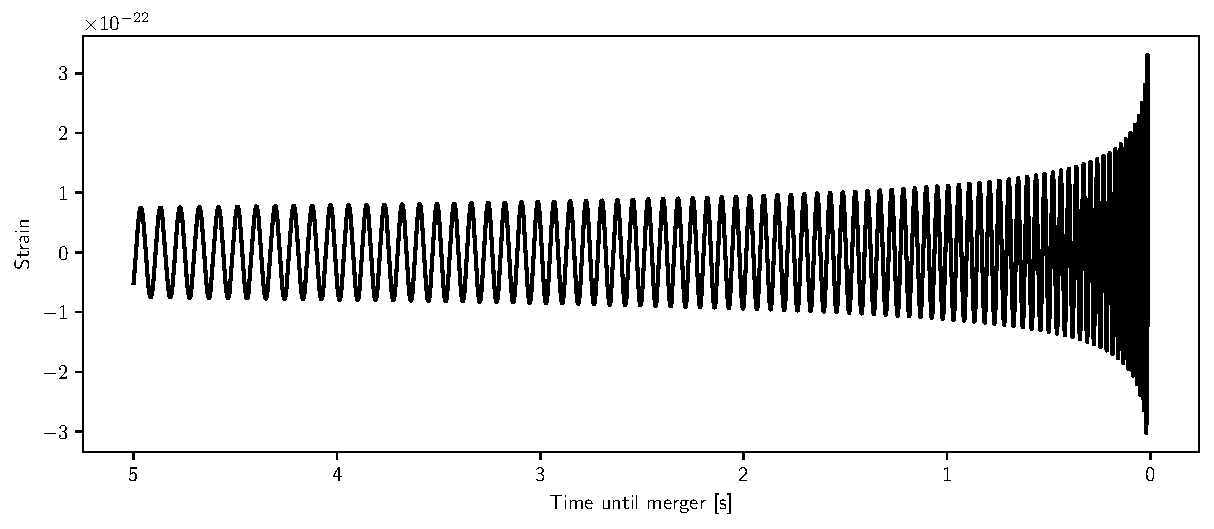
\includegraphics[width=\textwidth]{chapters/foundations/sections/gw/images/linear_waveform.pdf}
	\caption[Plus polarization waveform linearized gravity]{The strain of the plus polarization of a \acrshort{gw} as calculated by \eqref{eq:linear_waveform}. The parameters of the waveform are $m_1=$ \SI{35}{M_\odot}, $m_2=$ \SI{30}{M_\odot}, $r=$ \SI{1000}{\mega\parsec}, and $\iota, \Phi_0, \theta=0$.}\label{fig:linear_waveform}
\end{figure}


\subsection{Post-Newtonian Formalism}\label{sec:pn}
In the previous subsection the main approximation made to derive the gravitational radiation is the assumption of a flat background when describing the source dynamics. In other terms, we assumed that the orbital dynamics are governed by Newtonian dynamics and the background curvature is independent of the speed at which the bodies are orbiting. However, in a gravitationally bound system, the orbital velocity depends on the separation of the two bodies. More specifically, by the virial theorem one finds $\lr{v/c}^2\sim R_S/r$, where $R_S$ is the Schwarzschild radius and $r$ is the separation of the two objects~\cite{Maggiore:2008aaa}. %page 236
Therefore, the core assumption does not hold.

To treat gravitationally bound systems, one needs to consider a generic metric. However, solving the full Einstein equations is difficult and often impossible. One option to simplify problems are post-Newtonian (\acrshort{pn}) approximations~\cite{Misner:1973aaa}, %page 1069
where the full equations are expanded in a small parameter $\epsilon$. For binary systems, we use $\epsilon\sim\lr{v/c}$ and demand $\left|T^{ij}\right| / T^{00}=\mathcal{O}\lr{\epsilon^2}$, i.e. the source is at most weakly stressed~\cite{Maggiore:2008aaa}. %page 239
Requiring invariance of the equations under time-reversal the expansion works out to
\begin{align}
g_{00} & = -1 & & + g^{\lr{2}}_{00} & + g^\lr{4}_{00} & & + g^\lr{6}_{00} & & +\ \dots & \nonumber\\
g_{0j} & = & & & \phantom{+}g^\lr{3}_{0j}  & & + g^\lr{5}_{0j} & & +\ \dots & \\
g_{ij} & = & & \hspace{0.2cm}\phantom{+}\delta_{ij} & + g^\lr{2}_{ij} & & + g^\lr{4}_{ij} & & +\ \dots & ,\nonumber
\end{align}
where $g^\lr{n}$ denotes terms $\sim \epsilon^n$~\cite{Maggiore:2008aaa}. %page 239
To work consistently, when $g_{00}$ is expanded to order $n$, $g_{0i}$ must be expanded to order $n-1$ and $g_{ij}$ to order $n-2$~\cite{Maggiore:2008aaa}. %page 239
Similarly, the energy-momentum tensor also needs to be expanded
\begin{align}
T^{00} & = {T^\lr{0}}^{00} + {T^\lr{2}}^{00} + \dots\nonumber\\
T^{0j} & = {T^\lr{1}}^{0j} + {T^\lr{3}}^{0j} + \dots\\
T^{ij} & = {T^\lr{2}}^{ij} + {T^\lr{4}}^{ij} + \dots.\nonumber
\end{align}
To obtain approximations these expressions can be inserted into the Einstein equation \eqref{eq:einstein} and terms of the same order in $\epsilon$ can be equated. A solution is known to be of $n$-th \acrshort{pn}-order when terms up to order $\epsilon^{2n}$ are kept. Therefore, equations of $x.5$ \acrshort{pn}-order exist.

To 1 \acrshort{pn} order explicit solutions depending on the energy-momentum tensor are given in section 5.1.4 of \cite{Maggiore:2008aaa}, under the usage of the DeDonder gauge which in the full theory is given by
\begin{equation}
\partial_\mu\lr{\sqrt{-g}g^\mn}=0,
\end{equation}
where $g$ is the determinant of $g_\mn$. For the computation one also needs to consider that for $v/c\ll 1$ the time derivatives are smaller than the spatial derivatives by a factor $\mathcal{O}\lr{\epsilon}$ and hence the flat spacetime d'Alembert operator is given by
\begin{equation}\label{eq:pn_dalembert}
\Box = -\frac{1}{c^2}\frac{\partial^2}{\partial t^2}+\nabla^2 = \lr{1+\mathcal{O}\lr{\epsilon^2}}\nabla^2,
\end{equation}
where $\nabla^2=\delta^{ij}\partial_i\partial_j$. From this it is immediately clear that these solutions can only be valid close to the source, as they have to be instantaneous potentials~\cite{Maggiore:2008aaa}.%page 240

For further computations it is beneficial to cast the Einstein equations into their relaxed form
\begin{equation}\label{eq:relaxed_einstein}
\Box k^\mn = \frac{16 \pi G}{c^4}\tau^\mn,
\end{equation}
where $\Box$ is the flat spacetime d'Alembert operator,
\begin{equation}
k^\mn = \sqrt{-g}g^\mn-\eta^\mn,
\end{equation}
and
\begin{equation}
\tau^\mn=-gT^\mn + \frac{c^4}{16\pi G}\Lambda^\mn.
\end{equation}
The tensor $\Lambda^\mn$ captures the curvature contributions of the deviation from flat spacetime to the energy-momentum tensor~\cite{Blanchet:2006aaa} %page 16
and an explicit expression is given in (5.74) and (5.75) of \cite{Maggiore:2008aaa}. For \eqref{eq:relaxed_einstein} to be an exact equivalent to the Einstein equations \eqref{eq:einstein}, one also needs to enforce the DeDonder gauge which is given by $\partial_\nu k^\mn=0$ in this formulation.

To obtain a \acrshort{pn} expansion, we can then write the metric $k^\mn$ in a formal expansion of $v/c\approx 1/c$
\begin{equation}
k^\mn = \sum_{n=2}^\infty\frac{1}{c^n} k^\mn_n,
\end{equation}
where $v/c$ is the small parameter and only written for bookkeeping. As before, the right hand side of \eqref{eq:relaxed_einstein} must be expanded in the same manner~\cite{Maggiore:2008aaa}%page 261
\begin{equation}
\tau^\mn=\sum_{n=-2}^\infty\frac{1}{c^n}\tau^\mn_n.
\end{equation}
Inserting these expressions into the relaxed Einstein equation, using \eqref{eq:pn_dalembert}, and equating terms of the same order in $1/c$ we obtain the recursive equation
\begin{equation}
\nabla^2k^\mn_n = 16 \pi G \tau^\mn_{n-4} + \partial^2_t k^\mn_{n-2}.
\end{equation}
When solutions $k_0$ and $k_1$ are known, the right hand side of the above equation is fully determined and one needs to invert the Laplace operator $\nabla^2$ to obtain higher order \acrshort{pn} solutions.

This inversion, however, is not trivial, as the usual Poisson-integral diverges for high \acrshort{pn}-orders~\cite{Maggiore:2008aaa}. %page 261
Instead, one can find a particular solution for some finite \acrshort{pn}-order by multiplying the right hand side by $r^B$, for $B$ negative and large enough in magnitude. One can then consider the result in the complex plane and study the pole for $B\uparrow 0$, which is well defined and omits a solution. For the general solution the homogeneous solution has to be added. See 5.3.2 of \cite{Maggiore:2008aaa} and 5.2 of \cite{Blanchet:2006aaa} for more detail. Importantly, these solutions depend on the energy-momentum tensor of the source, but are only valid close to the source.

To get the radiation of the far field, we can consider the Post-Minkowskian (\acrshort{pm}) expansion. Since we are considering the region outside of the source, we are looking for vacuum solutions, i.e. $T^\mn=0$. In this case, the relaxed Einstein equation \eqref{eq:relaxed_einstein} simplifies to
\begin{equation}
\Box k^\mn = \Lambda^\mn.
\end{equation}
Outside the source the curvature will be small and we can expand in $R_s/r\sim G/r$. In a slight abuse of notation we write
\begin{gather}
k^\mn = \sum_{n=1}^\infty G^n k_n^\mn\\
\Lambda^\mn = N^\mn\left[k,k\right] + M^\mn\left[k,k,k\right]+\dotsc ,
\end{gather}
where $N^\mn$ and $M^\mn$ are tensors of quadratic and cubic order in $G$, respectively. Equating terms of the same order in $G$ leads to
\begin{equation}\label{eq:pm_wave_eq}
\Box k^\mn_n = \Lambda^\mn_n\left[k_1, \dotsc, k_{n-1}\right],
\end{equation}
where $\Lambda^\mn_n$ is the sum of all tensors $N^\mn,\ M^\mn,\ \dotsc$ of order $n$ in $G$.

In \eqref{eq:pm_wave_eq} we find another recursive relation, where higher order terms are determined from lower order ones. So once a solution $k^\mn_1$ is known, in principle all higher order solutions can be determined.

To find a solution to $k^\mn$ we observe that $\Lambda_1=0$ and write $k^\mn_1$ in a multipole expansion. Once the gauge condition is enforced, one can obtain solutions that depend on six families of multipole moments. See (5.95) to (5.101) in \cite{Maggiore:2008aaa} for explicit expressions. However, these multipole moments are still arbitrary functions, as they know nothing about the source of the radiation yet.

Iterating $k_1$ to find higher order solutions is again not trivial. In principle the right hand side of \eqref{eq:pm_wave_eq} is determined by all lower order solutions $k_1, \cdots, k_{n-1}$. So the task is in inverting the d'Alembert operator $\Box$. Notice that since the expansion is not in terms of $v/c$ anymore the d'Alembert operator must be inverted, rather than the Laplace operator. The solution to the problem is very similar to the solution used for the \acrshort{pn}-expansion. We find a particular solution by truncating the multipole expansion of $k^\mn_1$ at the desired order and multiply $\Lambda^\mn_n$ by $r^B$, with $B$ now positive and sufficiently large to cancel all factors $1/r$ in the multipole expansion. We then use the analytic continuation again and add the homogeneous solution to obtain the most general one. See 5.3.1 of \cite{Maggiore:2008aaa} or 4.1 of \cite{Blanchet:2006aaa} for more detail.

To determine the multipole moments of the \acrshort{pm} solutions, one observes that the \acrshort{pn} and \acrshort{pm} solutions have an overlapping region of validity~\cite{Blanchet:2006aaa}. Therefore, one uses the \acrshort{pn} solutions, which are determined by the energy-momentum tensor of the source, to fix the multipole moments of the \acrshort{pm} solutions. To do so, the \acrshort{pn} potentials are written as a multipole expansion and the \acrshort{pm} solitions are re-rexpanded in terms of powers of $1/c$. Finally, terms of the same order are equated. The explicit expressions are given in (85) - (90) of \cite{Blanchet:2006aaa}.

With this, the metric in the far region has in principle been determined. To find the actual waveform emitted by some physical system, one can follow a very similar approach to the one used in \autoref{sec:linear_gravity}. A binary system is well approximated by a sum of two delta functions\footnote{Using delta functions will actually lead to divergencies at high \acrshort{pn}-order. For this reason some regularization has to be applied. See section 8 of \cite{Blanchet:2006aaa} for details.} in the energy-momentum tensor. Using this energy-momentum tensor, one can find the metric in the near region of the source to determine the orbital energy $E$. On the other hand, it can be used to determine the metric in the far region, which can in turn be integrated to obtain the luminosity $L_{\text{\acrshort{gw}}}$ of the source. Under the assumption that the system loses energy only through gravitational radiation, we can use the equation
\begin{equation}
-\frac{\diff E}{\diff t} = L_{\text{\acrshort{gw}}}
\end{equation}
to obtain the orbital phase of the binary system.

For the case of linearized gravity discussed in \autoref{sec:linear_gravity} the orbital energy was known from Newtonian dynamics. In the \acrshort{pn} approximation it needs to be calculated. To do so, one inserts the \acrshort{pn} metric into the geodesic equation \eqref{eq:geodesic_equation} to obtain the equations of motion of the two orbiting bodies. From this one can find the orbital energy. Explicit expressions can be found in \cite{Blanchet:2006aaa}, equation (115) gives the generic metric to $3$ \acrshort{pn}-order, (168) gives the equation of motion of a binary system to $3.5$ \acrshort{pn}-order, (170) gives the orbital energy to $3$ \acrshort{pn}-order, and (194) gives the energy to $3$ \acrshort{pn}-order assuming circular orbits.

The luminosity can be directly computed from the metric by integration. See section 3.5 of \cite{Maggiore:2008aaa} or section 6 and section 10.2 of \cite{Blanchet:2006aaa} for details. Explicit expressions at $3.5$ \acrshort{pn}-order are given in (5.257) of \cite{Maggiore:2008aaa} and (231) of \cite{Blanchet:2006aaa}. The resulting phase to $3.5$ \acrshort{pn}-order is given in (235) of \cite{Blanchet:2006aaa}.

To obtain the waveform, one can project the metric $g_{ij} - \delta_{ij}$ into the \acrshort{tt}-frame. The metric $g_{ij}$ is the desired \acrshort{pn}-approximation, the derivation of which was discussed above. The polarizations can be read of. Explicit expressions were derived in \cite{Blanchet:1996pi, Arun:2004ff} and can be found in (237) - (241) of \cite{Blanchet:2006aaa}. To get the actual waveform, the time dependent phase to highest known \acrshort{pn}-order should be inserted.

The discussion above is meant as a high-level overview of how \acrshort{pn}-waveforms can be obtained. A more detailed overview, including mathematical details, is given in \cite{Blanchet:2006aaa}. Notably, this discussion excluded spin effects of the binary system and its constituents. Discussions including spin can be found for instance in \cite{Damour:2001tu, Blanchet:2004ek, Faye:2006gx, Blanchet:2006gy, Damour:2007nc}.


\subsection{Waveform Models}
The waveforms discussed in subsections \ref{sec:linear_gravity} and \ref{sec:pn} are, by construction, only valid during the inspiral, even though high order \acrshort{pn} waveforms remain accurate until a few cycles before the merger of the two objects~\cite{Blanchet:2006aaa, Santamaria:2010yb}. %page 85, last paragraph
However, the emitted energy scales to high power with the orbital frequency of the two merging objects, as can be seen from \eqref{eq:luminosity_linear} to linear order and from (231) of \cite{Blanchet:2006aaa} to $3.5$ \acrshort{pn}-order. Therefore, the evolution of the waveform close to merger can be of high importance for detection.

This subsection gives an overview of the three most prominently used waveform-model families and their variants. All of them model the entire orbital evolution from inspiral, over merger, to ringdown (\acrshort{imr}), in the parameter regions where they are valid. To be able to represent the merger phase, all of them rely on numerical relativity (\acrshort{nr}) simulations, which solve the Einstein equations numerically. These simulations are the most accurate tools available to solve the highly non-linear interactions but running them requires enormous amounts of computational power. Generating a waveform encompassing the final few orbits and the merger for a single binary system using \acrshort{nr} can take days or even weeks, depending on the initial conditions and type of binary system~\cite{Hannam:2009rd}. Therefore, it is often not viable to use the resulting waveforms in data analysis methods discussed in section \ref{sec:cbc_searches} directly. The waveform models below are constructed to overcome this issue by combining the accurate \acrshort{nr} waveforms with analytical approximations.

Instead of writing the \acrshort{gw} polarizations as individual functions, one can also define a single complex strain
\begin{equation}
H\coloneqq h_+ + i h_\times,
\end{equation}
which can be decomposed using spherical harmonics~\cite{Thorne:1980ru, Dhurkunde:2022aek}
\begin{equation}\label{eq:complex_waveform}
H=\sum_{l\geq 2}\sum_{m=-l}^l Y^{-2}_{lm}\lr{\iota, \Phi_0}h_{lm}\lr{\tau, r, \kappa},
\end{equation}
where
\begin{equation}
h_{lm}\lr{\tau, r, \kappa} = A_{lm}\lr{\tau, r, \kappa} e^{-i\Phi_{lm}\lr{\tau, \kappa}}.
\end{equation}
$\kappa$ represent all parameters that describe the source itself and which do not depend on the location at which one observes the radiation. Waveform models usually describe the amplitude evolution $A_{lm}$ and the phase evolution $\Phi_{lm}$. If a waveform model is capable of modeling these quantities for $(l, m) \neq (2, \pm 2)$, one speaks of a model that is capable of simulating higher order modes (\acrshort{hm}).


\subsubsection{Effective One-Body Waveform-Family}
Effective one body (\acrshort{eob}) waveforms were one of the first \acrshort{gw} approximants that could model not only the inspiral but also the merger and ringdown. The formalism was introduced in \cite{Buonanno:1998gg} and maps the two body problem of a \acrshort{bbh} system onto that of a test particle moving in an effective external metric. To that end, a Hamiltonian is constructed which is supplemented with a radiation-reaction force. It takes the \acrshort{pn} approximation as a starting-point to express the Hamiltonian and then expresses it as well as the radiation-reaction force in a resummed form, where the functions are non-polynomial~\cite{Damour:2008te}. An introduction to the resummation is given in 14.1 of \cite{Maggiore:2018aaa}. This resummation can then be extended by adding free parameters that model non-perturbative effects~\cite{Damour:2001tu, Damour:2002vi, Damour:2007xr}. The \acrshort{eob} formalism models the inspiral and merger by fitting the free parameters to \acrshort{nr} and then attaches an analytical model for the ringdown.

The first full \acrshort{imr} waveform from the \acrshort{eob} family was derived in \cite{Buonanno:2000ef}. Initially it modeled only non-spinning \acrshort{bbh}s but was later extended to the spinning case in \cite{Buonanno:2005xu, Barausse:2009aa}. The early models were solely based on analytic calculations. However, with the breakthrough in \acrshort{nr} in 2005~\cite{Maggiore:2018aaa, Pretorius:2005gq, Campanelli:2005dd, Baker:2005vv} accurate ground-truths became available, which could be used to constrain the free parameters that extend the \acrshort{eob} models~\cite{Buonanno:2007pf, Damour:2008te}. These models were incrementally improved~\cite{Damour:2009kr, Buonanno:2009qa} and extended to include higher order modes, aligned spins, and precession~\cite{Barausse:2009xi, Pan:2009wj, Pan:2011gk, Pan:2013rra}. To keep track of the capability of these models, a naming scheme was introduced. Waveforms of this family carry an ``\acrshort{eob}'' in their name, which is usually followed by ``\acrshort{nr}'' to signify that the model coefficients were tuned to \acrshort{nr} simulations. A leading ``S'' informs the user about the capability of the model to represent (anti-)aligned spins. Afterwards a version number is tagged onto the string. The first model named this way is known as ``SEOBNRv1'' and was introduced in \cite{Taracchini:2012ig}, ``SEOBNRv2'' is the model described in \cite{Taracchini:2013rva, LIGOScientific:2016vlm}, ``SEOBNRv3'' the one described in \cite{Pan:2013rra, LIGOScientific:2016vlm}, and ``SEOBNRv4'' in \cite{Bohe:2016gbl}. At the time of writing, the \acrshort{eob} model that encompasses the most orbital dynamics is ``SEOBNRv4PHM'', which can account for higher order modes and precession at the same time~\cite{Ossokine:2020kjp}. The \acrshort{eob} models are formulated as a set of differential equations, that need to be solved for given parameters, which can be prohibitively slow depending on the application~\cite{LIGOScientific:2016vlm}. They are also formulated in the time domain, wheras data analysis usually requires the waveform in the frequency domain. For these reasons, \acrshort{eob} models are often sped up by building reduced order models in the frequency domain~\cite{Purrer:2014fza, Purrer:2015tud}.


\subsubsection{Phenom Waveform-Family}
The phenomelogical -- short Phenom -- waveform-family was introduced in \cite{Ajith:2007qp}. At the core, their method matches the analytic \acrshort{pn}-waveform that describes the inspiral with the more accurate \acrshort{nr}-waveform during merger to produce a finite amount of hybrid waveforms. Afterward, the hybrid waveforms are fit to a phenomenological parametrized model which can in turn be mapped to the physical parameters of the binary system~\cite{Santamaria:2010yb}. The resulting model is fast to evaluate, highly accurate, and usually native to the frequency domain.

Since the initial paper, which focused on non-spinning \acrshort{bbh}s in a mass range of \SI{30}{M_\odot} to \SI{130}{M_\odot}, many different versions of the waveform model have been released. The work of \cite{Ajith:2009bn} introduced a Phenom-waveform model that is capable of modeling \acrshort{bbh}s, the spins of which are (anti-)aligned with the orbital angular momentum. Through \cite{Schmidt:2012rh, Hannam:2013oca} waveform models that can take precession effects of the emitting binary into account were introduced and dubbed PhenomP, where the ``P'' signifies the ability to represent precessing systems. The PhenomP model was used during data analysis of the first detected \acrshort{gw}~\cite{LIGOScientific:2016aoc, LIGOScientific:2016vlm, LIGOScientific:2019hgc}. The authors of \cite{London:2017bcn} introduced a model that can account for higher multipoles (``PhenomHM''), which was combined with an updated version of the precessing waveform model~\cite{Khan:2018fmp} to obtain a waveform model that can represent both effects~\cite{Khan:2019kot} (``PhenomPv3HM''). The underlying model was also revised multiple times over the years. The evolving non-precessing approximants were called ``PhenomB''~\cite{Ajith:2009bn}, ``PhenomC''~\cite{Santamaria:2010yb}, and ``PhenomD''~\cite{Husa:2015iqa, Khan:2015jqa}. The most recent version, skipping many letters in between, is the ``PhenomX'' waveform model~\cite{Pratten:2020fqn}, which has a version that allows for the computation of higher order multipoles called ``IMRPhenomXHM''~\cite{Garcia-Quiros:2020qpx}, and a version that includes both higher order multipoles and precession effects, known as ``IMRPhenomXPHM''~\cite{Pratten:2020ceb}. The prefix ``IMR'' signifies that the waveform models the full inspiral-merger-ringdown. The postfix ``HM'' signifies that higher order multipoles can be computed.


\subsubsection{Numerical Relativity Surrogate Waveform-Family}
By now hundreds of \acrshort{nr} simulations are available that span large parts of the expected parameter space for \acrshort{bbh} mergers~\cite{Boyle:2019kee, Healy:2022wdn}. The resulting waveforms are the most accurate predictions of the emitted radiation of a merging binary system that are available to us. \acrshort{nr} surrogate models leverage the existing catalogs of \acrshort{nr} simulations to interpolate between them. They are typically more accurate than the approximate methods described above but are only valid in the limited parameter regions that are covered by the underlying simulations~\cite{Setyawati:2019xzw}.

The first surrogate model was introduced in \cite{Blackman:2015pia} and used non-spinning waveforms produced by the Spectral Einstein Code~\cite{Scheel:2014ina, Szilagyi:2014fna}. The model was later extended to include precession~\cite{Blackman:2017dfb} and more parameters~\cite{Blackman:2017pcm, Varma:2018aht}. Currently the model named ``NRSur7dq4''~\cite{Varma:2019csw} is used in state-of-the-art analyses~\cite{LIGOScientific:2021djp}, where ``7dq4'' signifies that the model is valid for a $7$ dimensional parameter space (6 spins + mass ratio) up to a mass ratio $q$ of $4$.
